Het paspoort waarmee een webserver aantoont dat die echt de enige echte is heet een certificaat\index{Certificaat} en net als een paspoort moet een certificaat door een instantie uitgegeven worden. Paspoorten worden uitgegeven door de gemeente (overheid) en certificaten door Certificate Authorities\index{Certificate Authority} (CA\index{CA}). Een certificaat bevat:
\begin{itemize}
\item De public key van de server
\item De domeinnaam waarvoor het certificaat geldig is
\item De geldigheidsduur
\item De handtekening (signature) van de CA
\end{itemize}

Een voorbeeld van een signature is te zien in figuur \ref{img:cert:letsencrypt}.

\begin{figure}[h]
\centering
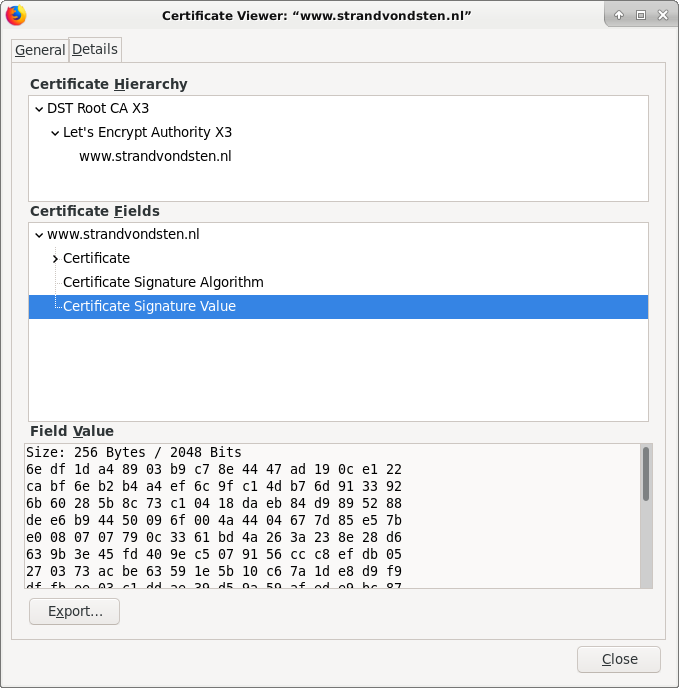
\includegraphics[width=0.8\textwidth]{Certificaat_LetsEncrypt.png}
\caption{Let's Encrypt certificaat}
\label{img:cert:letsencrypt}
\end{figure}

Een webserver heeft dus zijn eigen private key en een certificaat ge\"installeerd staan. Het stuurt zijn certificaat op aan een gebruiker (browser), die controleert het certificaat en als het goed bevonden wordt gebruikt het de public key uit het certificaat om een encrypt bericht aan de server te sturen die dat bericht can decrypten met zijn private key.
